\documentclass[a4paper,11pt]{scrartcl}
\usepackage[paper=a4paper,left=25mm,right=25mm,top=25mm,bottom=40mm]{geometry}
\usepackage[T1]{fontenc}
\usepackage[utf8]{inputenc}
\usepackage[ngerman]{babel}
\usepackage{graphicx}
\usepackage{url}
\usepackage{hhline}
\usepackage[usenames,dvipsnames]{xcolor}
\usepackage{fancyhdr}
\usepackage{verbatimbox}
\usepackage{tikz}
\usepackage{enumitem}
\usepackage{enumerate}
\usepackage{wasysym}

\newcounter{gesamtpunkte}
\setcounter{gesamtpunkte}{0}

\newcounter{aufgabenzaehler}
\setcounter{aufgabenzaehler}{1}

\newcommand{\aufgabe}[2]{\subsubsection*{\theaufgabenzaehler. Aufgabe (#1 Punkte)}#2\stepcounter{aufgabenzaehler}\addtocounter{gesamtpunkte}{#1}}

%% Lösung
%\newcommand{\aufgabe}[2]{\subsubsection*{\theaufgabenzaehler. Aufgabe (#1P)}#2\subsubsection*{Lösung:}\stepcounter{aufgabenzaehler}\addtocounter{gesamtpunkte}{#1}}

\pagestyle{fancy}
\lhead{GBS Schulen gGmbH}
\chead{I4A, 2. Schulaufgabe, AME}
\rhead{03. Mai 2018}
\lfoot{} \cfoot{\pagemark} \rfoot{}
\renewcommand{\headrulewidth}{0.4pt}

\makeatletter
\AtEndDocument{
    \write\@auxout{\string\gdef\string\@gesamtpunkte{\arabic{gesamtpunkte}}}
}

\newcommand*\gesamtpunkte{%
\@ifundefined{@gesamtpunkte}{??}{\@gesamtpunkte}%
}
\makeatother

\begin{document}
\subsubsection*{Gesamtpunkte: \gesamtpunkte}
\aufgabe{50}{
    Erstellen Sie eine Android-App wie in folgender Abbildung dargestellt:
    \begin{figure}[h]
        \centering
        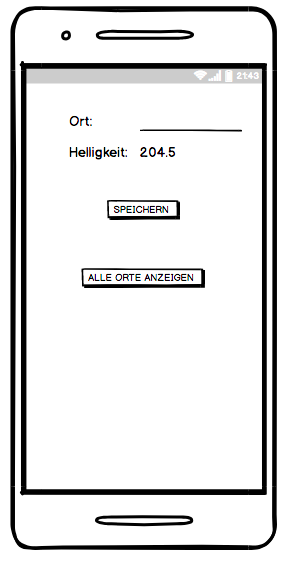
\includegraphics[width=6cm]{./App1.png}
    \end{figure}
    \\
    Im Texteingabefeld soll der aktuelle Ort eingegeben werden. Stellen Sie mit Hilfe des Lichtsensor die aktuelle Helligkeit dieses Ortes dar. Klickt der Benutzer auf \textit{SPEICHERN} soll der eingegeben Ort mit der aktuellen Helligkeit und dem aktuellen Zeitpunkt gespeichert werden. Erstellen Sie dazu geeignete Modellklassen. 
}
\newpage
\aufgabe{30}{
    Klickt der Benutzer auf \textit{ALLE ORTE ANZEIGEN}, soll eine neue \textit{Activity} gestartet werden. Alle gespeicherten Orte sollen in einer Liste wie folgt dargestellt werden:
    \begin{figure}[h]
        \centering
        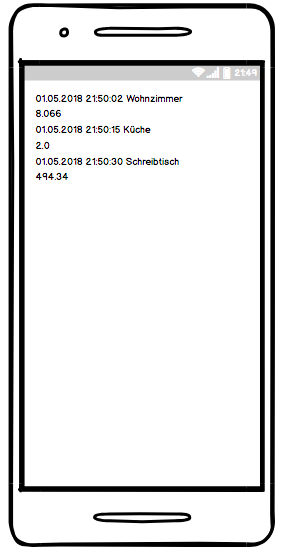
\includegraphics[width=6cm]{./App2.png}
    \end{figure}
}
\aufgabe{20}{
    Klickt der Benutzer auf einen Listeneintrag und die Helligkeit dieses Eintrages ist geringer als 200 soll für 5 Sekunden das Blitzlicht der Kamera wie bei einer Taschenlampe leuchten.
}



\end{document}